\chapter{Gestione e struttura del database}
% \section{Gestione e struttura del database}

\section{Progettazione iniziale}
% \subsection{Progettazione iniziale}
Una delle prime attività del progetto è stata la progettazione della base di
dati, e fin dall'inizio era chiaro che non si sarebbe trattato di uno schema
molto complesso. Infatti con sole tre tabelle si riesce a descrivere in modo
appropriato l'ambiente nel quale risiede il progetto.
\subsection{Schema Concettuale}
% \subsubsection{Schema Concettuale}
 La tabella principale e da cui si è partiti è
quella delle stazioni, che presenta una chiave primaria (Key), un nome che
identifica la stazione, l'indirizzo cioè il nome della via nella quale risiede, la
posizione (formata da due coordinate geografiche di latitudine e longitudine che
sono realizzate mediante due variabili double), e
una descrizione opzionale formata da un testo. La
stazione possiede poi una Tipologia. Tramite colloquio con il commitente dott.
Marco  Aceti si è appreso come le stazioni di ricarica possono essere
raggruppate
in diversi insiemi dovuti al servizio vero e proprio che viene fornito oltre a
quello della ricarica. Esistono stazioni nelle quali è possibile noleggiare bici
elettriche e altre dove si può portare la propria bici per effettuare della manutenzione.
Dunque la tabella TipoStazione contiene per ogni riga una diversa tipologia di
stazione, formata dalla combinazione dei diversi servizi appena descritti, in
quanto ovviamente esistono negozi che propongono più servizi contemporaneamente.
Ogni istanza di questa tabella oltre a possedere una chiave che la identifica,
è caratterizzata dal nome (cioè la tipologia) e da un numero intero chiamato
\textit{Colore} che viene utilizzato all'interno dell'applicazione per fornire un colore
diverso a ogni tipologia in modo da rendere più semplice agli utenti
l'identiticazione di ciò che può interessare loro. Nello schema deve poi essere
presente una tabella che tenga traccia degli utenti. Si presti attenzione che
questa tabella è diversa da quella gestita da Firebase relativa agli accessi e
alle tipologie di utenti descritta nel precedente capitolo: qui vengono presi in
considerazione il nome dell'utente e oltre alla chiave per identificarlo la
propria preferenza sulla tipologia di mappa scelta. Non si esclude che in futuro
si possano aggiungere ulteriori campi relativi a nuove preferenze che
potrebberero essere scelte. Nella figura \ref{schemaEr} è mostrato lo schema Entità-Relazione
del progetto. Si noti come una stazione debba per forza appartenere alla
relazione Inserimento in quanto deve essere stata inserita da qualcuno, ma un
utente può non appartenere a tale relazione in quanto può tranquillamente
utilizzare l'app per conoscere la posizioni di stazioni senza mai inserirne nessuna.

\begin{figure}[ht!]
    \centering
    {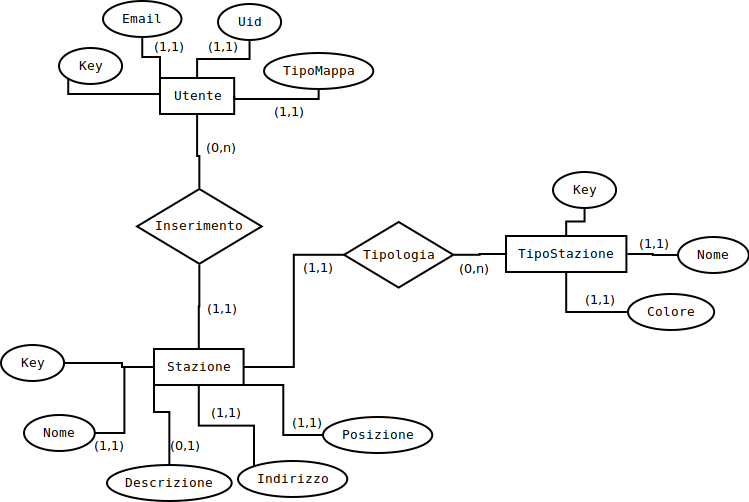
\includegraphics[scale=0.5]{ERTesi.png}}
    \caption{Schema Concettuale del progetto}
    \label{schemaEr}
\end{figure} 

\subsection{Schema Logico}
% \subsubsection{Schema Logico}
Data la semplicità dello schema Entità-Relazione la fase di progettazione logica
è stata anch'essa priva di ostacoli. Si è posta particolare attenzione alle
relazioni \textit{Inserimento} e \textit{Tipologia} perchè sarebbero potute diventare delle
tabelle ma dato che entrambe sono del tipo (1,1) verso (0,n) si è scelto di
renderle degli attributi della tabella Stazione, diventando quindi chiavi
esterne (figura \ref{schemaLogico}). 

\begin{figure}[ht!]
    \centering
    {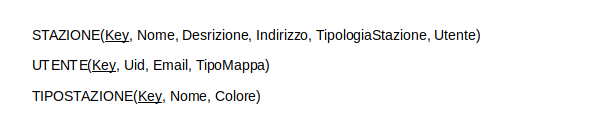
\includegraphics[width=15cm]{LogicoTesi.png}}
    \caption{Schema Logico del progetto}
    \label{schemaLogico}
\end{figure} 

\section{Gestione dati in Firebase}
% \subsection{Gestione dati in Firebase}
Quando si crea un progetto nella propria Firebase Console una delle prime
importanti operazioni è quella di scegliere la tipologia di database. Il
servizio Google infatti offre due possibili alternative: il Realtime Database
oppure il Cloud Firestore. Fino alla fine del 2018 la prima opzione era anche
l'unica disponibile e consiste in una soluzione efficiente, a bassa latenza per
applicazioni mobili che richiedono la sincronizzazione di stato tra client
diversi in un tempo paragonabile alle prestazioni di un sistema real time. Il
secondo, disponibile da minor tempo, è stato sviluppato per migliorare
ulteriormente il suo predecessore, cambiando anche il modo in cui i dati vengono
organizzati all'interno dello storage. Entrambe queste soluzioni sono database
costruiti per tecnologie NoSQL, dunque non sfruttano le classiche tabelle dove
ogni riga di una tabella è un record che contiene sempre lo stesso numero e
tipologia di attributi. La tipologia Realtime immagazzina i dati in un unico
grande albero JSON. Questo comporta una relativa facilità nell'inseriemento dati
soprattutto se di ridotte dimensioni, ma nel momento in cui la grandezza e
complessità del database non sono più banali diventa difficile organizzare una
struttura gerarchica. La tipologia Cloud immagazzina invece i dati in documenti
chiamati \textit{collections}, ne segue quindi che essa fa parte delle cosiddette
basi di dati orientate al documento. Strutture dati modeste sono molto facili
da inserire (in modo simile al metodo visto prima tramite JSON) e se queste
diventano complesse e di grandi dimensioni usando collezioni e sotto-collezioni si
può facilmente organizzare il tutto senza perdere in efficienza. Considerando
invece le funzionalità relative all'effettuare query, per il Realtime Database è
possibile filtrare o ordinare dati in una sola query, mentre per il Cloud
Firestore è possibile effettuare entrambe le operazioni nella stessa query.
Inoltre nella prima tipologia il risultato è sempre un albero JSON che contiene
tutti i dati, dunque le dimensioni possono assumere una certa importanza, mentre
nella seconda le performance della query sono proporzionali alla grandezza del
risultato e non dell'intera struttura. A seguito di queste considerazioni si è
quindi deciso, benchè il progetto non presenti strutture particolarmente
complesse, di utilizzare Cloud Firestore. 

\section{Utilizzare il Cloud Firestore}
% \subsection{Utilizzare il Cloud Firestore}
In questa sezione verranno prese in considerazione le modalità con cui si sono
svolte le query all'interno dell'applicazione. Prima di tutto è doveroso dire
che per effettuare interrogazioni al proprio database è necessario importare nel
proprio progetto il pacchetto \textit{cloud\_firestore}. Grazie a questo si ha
accesso all'oggetto Firestore che permette all'app di comunicare con il database
realtime sul cloud.
\subsection{Ottenere tutti gli elementi di una collezione}
% \subsubsection{Ottenere tutti gli elementi di una collezione}
Quando si visualizza la pagina della mappa, è necessario visualizzare tutte le
stazioni presenti nel database senza applicare dei filtri. Bisogna quindi
effettuare il corrispettivo di una SELECT ALL nel linguaggio SQL. 
\begin{figure}[!h]
    \centering
    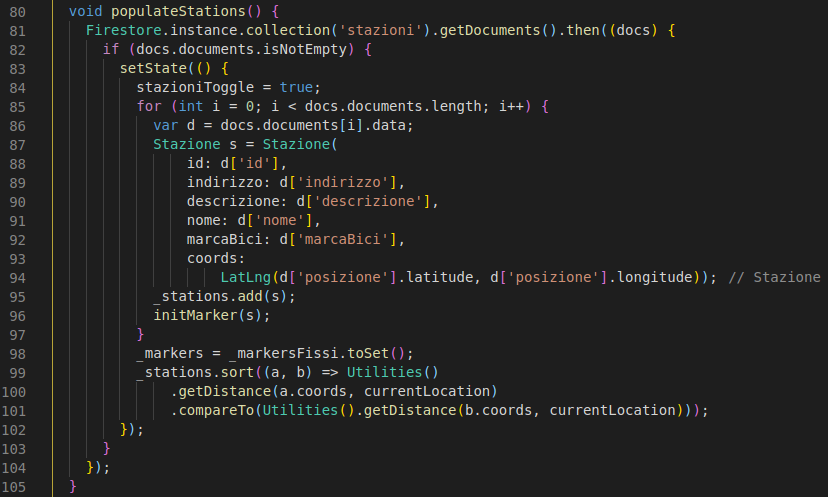
\includegraphics[width=13cm]{query1.png}
    \caption{La funzione populateStations che permette di ottenere tutte le stazioni presenti nel database}
    \label{query1}
\end{figure}
In figura \ref{query1} si può quindi vedere il metodo populateStations che viene
chiamato nel momento in cui l'utente termina la propria autenticazione e
raggiunge la pagina della mappa. Sulla firebase console del progetto è presente
la collezione \textit{stazioni}, a cui si fa accesso alla linea 81 tramite il
metodo \verb|Firestore.instance.collection('stazioni').getDocuments()|. Questo
metodo è di tipo Future (si rimanda al capitolo su Flutter e Dart), e quindi
necessita del metodo \verb|then()| per accedere ai dati inviati in modo
asincrono. Una volta connessi al database e ottenuti i documenti, si controlla
che essi non siano di lunghezza nulla (tramite il campo
\verb|docs.document.isNotEmpty|). Se si è ottenuta almeno una stazione si
procede quindi a creare un oggetto di tipo Stazione per ogni elemento nella
firebase console tramite il suo costruttore, e si inserisce dunque l'oggetto
nella lista di stazioni \verb|_stations|. Si procede poi con la funzione
\verb|initMarker| che inizializza ogni stazione rendendola un marker
visualizzabile nella mappa e si ordinano poi le stazioni in base alla vicinanza
dalla posizione attuale dell'utente tramite una classe (Utilities) creata per
sfruttare funzioni quali l'ordinamento o il controllo di alcuni campi.

\subsection{Ottenere dati filtrati da una collezione}
% \subsubsection{Ottenere dati filtrati da una collezione}
Ci sono diversi casi all'interno dell'applicazione in cui è necessario ottenere
uno specificio documento o un gruppo selezionato da una collezione. Per esempio
per ottenere la preferenza dell'utente rispetto alla tipologia di mappa che
vuole visualizzare bisogna ottenere uno e un solo documento nella collezione
users. \\
\begin{figure}[!h]
    \centering
    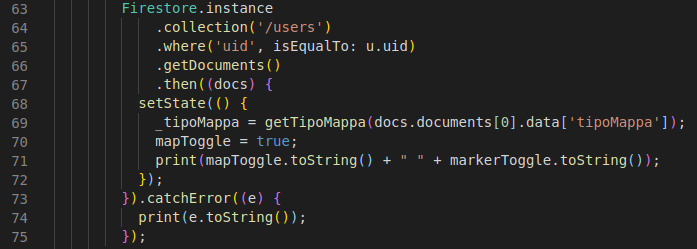
\includegraphics[width=12cm]{query2.png}
    \caption{}
    \label{query2}
\end{figure}
Nella figura \ref{query2} si accede alla collezione users nel solito modo visto
anche precedentemente, ciò che cambia è che ora si introduce anche il metodo
\verb|where()| che prende come primo argomento una stringa indicante il nome del
campo su cui si vuole effettuare la selezione, e un secondo argomento che indica
il tipo di confronto che si vuole fare, in questo caso un \textit{isEqualTo}
(tra gli altri sono presenti anche \textit{isGreaterThan} e
\textit{isLessThan}). Una volta ottenuto l'utente che ha lo stesso \textit{id}
dell'user attuale si può quindi accedere al suo campo \verb|tipoMappa| e
tramite un metodo apposito convertire la stringa ottenuta nella tipologia di
mappa desiderata. Si noti anche il metodo \verb|catchError()| che è sucessivo al
\verb|then()| relativo ai documenti della collezione: in caso di un qualunque errore di
connessione l'app non smette di funzionare ma cattura l'eccezione ottenuta e va
avanti nell'esecuzione di codice. Se si volesse effettuare filtraggio di dati su
più campi sarebbe necessario banalmente continuare ad aggiungere metodi
\verb|where| ai documenti ottenuti indicando i nomi dei campi e la condizione
che si vuole applicare.


